%!TEX program = xelatex
\documentclass{beamer}

\usepackage{blindtext}
\usepackage{amsmath}
\setbeamercovered{highly dynamic}

\newcounter{saveenumi}
\newcommand{\seti}{\setcounter{saveenumi}{\value{enumi}}}
\newcommand{\conti}{\setcounter{enumi}{\value{saveenumi}}}

\resetcounteronoverlays{saveenumi}

\usetheme{Execushares}

\title{Classification of text using Association Rule mining with Critical Relative Support based pruning}
\subtitle{ICACCI, Jaipur}
\author{Saurabh Mathur (VIT, Vellore)}
\date{September 23, 2016}

\setcounter{showSlideNumbers}{1}

\begin{document}
	\setcounter{showProgressBar}{0}
	\setcounter{showSlideNumbers}{0}

	\frame{\titlepage}
	\begin{frame}
		\frametitle{Contents}
		\begin{enumerate}
			\item Introduction \\ \textcolor{ExecusharesGrey}{\footnotesize\hspace{1em} The problem statement}
			\item Background  \\ \textcolor{ExecusharesGrey}{\footnotesize\hspace{1em} Other approaches to solve the problem}
			\item Proposed Idea  \\ \textcolor{ExecusharesGrey}{\footnotesize\hspace{1em} Our approach to solve the problem}
			\item Results \& Conclusions \\ \textcolor{ExecusharesGrey}{\footnotesize\hspace{1em} Some closing thoughts}
		\end{enumerate}
	\end{frame}

	\setcounter{framenumber}{0}
	\setcounter{showProgressBar}{1}
	\setcounter{showSlideNumbers}{1}
	
	\section{Introduction}
		
		\begin{frame}
			\frametitle{Association Rules}
			\begin{center} \LARGE{ \texttt{ \{Bread, Milk\} => \{Butter\} } }  	\end {center}
			\textcolor{ExecusharesGrey}{\footnotesize\hspace{1em} The Apriori algorithm \super{[1]} is a way to generate such rules from transaction data}
		    		
		\end{frame}
		
		
		\begin{frame}
			\frametitle{Problem Statement}
			\begin {center} \huge{Find the minimal set of interesting association rules \textit{from text}}  
			\end {center}
			
		    		
		\end{frame}
		 
		
		\begin{frame}
			\frametitle{The dataset}
			\begin {columns}
			\column{0.5\textwidth}
			 \large{BBC Insights dataset \super{[5]} } \\ \medskip
			 
			 \begin{table}
			 \begin{tabular}{r c}
			 2004-2005 & \textcolor{ExecusharesGrey}{ Time period } \\
			 2,225 & \textcolor{ExecusharesGrey}{ Documents } \\
			 5 & \textcolor{ExecusharesGrey}{ Categories } \\
			 
			 \end{tabular}
			 \end {table}
			\column{0.5\textwidth}
			
\includegraphics[width=\textwidth]{bbc.png}
			\end {columns}
		    		
		\end{frame}
		
	\section{Background}
	\begin{frame}
		\frametitle{Literature Survey}
		
		\begin{table}
			 \begin{tabular}{p{4cm} p{6cm}}
			 \textcolor{ExecusharesGrey}{Citation} & \textcolor{ExecusharesGrey}{tl;dr} \\
			 Rakesh Agrawal and Ramakrishnan Srikant; 1993 \super{[1]} \smallskip & Apriori Algorithm proposed. \\ 
			 
			 Zailani Abdullah, et al.; 2011 \super{[2]} \smallskip & Proposed a metric (CRS) to remove uninteresting rules. \\
			 Gayathri, K.; Marimuthu, A.; 2013 \super{[3]} \smallskip & 
Text classification performance is independent of size of feature space in most cases. \\
			Kulkarni et al. 2012 \super{[6]} & Feature co-occurrence and association are can be used for classification \\
			 Kadhim, A.I.; Cheah, Yu.-N; 2014 \super{[4]} \smallskip & Term weighing and NLP  reduce the dimensionality of the feature space\\
			 
			 \end{tabular}
			 
			 
		\end {table}
		
	\end{frame}
	\section{Proposed Idea}
		\begin{frame}
			\frametitle{Flowchart - Part 1}
			\begin {center}
			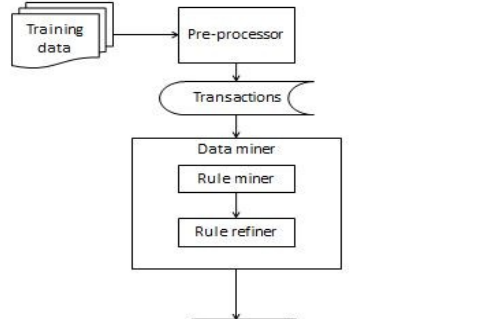
\includegraphics[scale=0.5]{flowchart1.png}
			\end {center}
		\end{frame}
		
		\begin{frame}
			\frametitle{Flowchart - Part 2}
			\begin {center}
			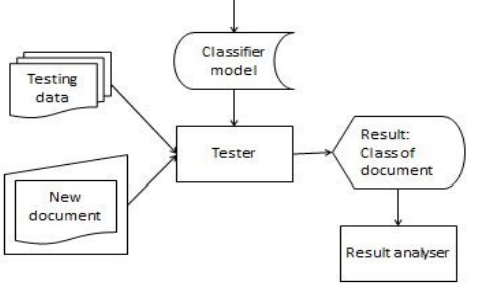
\includegraphics[scale=0.6]{flowchart2.png}
			\end {center}
		\end{frame}

		\begin{frame}
			\frametitle{Pre-Processing}
			\LARGE{Convert text document to transaction format} \\
			\textcolor{ExecusharesGrey}{\footnotesize\hspace{1em}{ Tokenizing. Stop word removal. POS Tagging. Stemming. Tf-Idf.   } }
			
			\LARGE{Find representative features} \\
			\textcolor{ExecusharesGrey}{\footnotesize\hspace{1em}{Features found only in a particular class } }
		    		
		\end{frame}
		
		\begin{frame}
			\frametitle{Rule mining}
			\begin{center}
			\LARGE{\texttt{ X => Y}} \\
			\end{center}
			
			$ Y \in Classes $ \\ 
			Classes = \{ Business, Entertainment, Politics, Sports, Technology \} 
		    		
		\end{frame}
		
		\begin{frame}
			\frametitle{Rule Filtering with CRS}
			Before applying CRS filtering, update support as -
			\begin{center}
			$ Mod_{Supp}(X=>Y) = (1-a)\cdot(1-b)\cdot(1-c)\cdot supp(X=>Y) $
			\end{center}
			
			Where, \\
			$a = \frac{\text{Number of documents of class Y}}{\text{Total number of documents}}$ \\ \smallskip
			$b = \frac{\text{Number of representative features of class Y}}{\text{Total number of documents}}$ \\ \smallskip
			$c = \frac{\text{Number of rules of class Y}}{\text{Total number of rules}}$
			
		    		
		\end{frame}
		

		
	\section{Results \& Conclusion}
	\begin{frame}
			\frametitle{Accuracy}
			\begin{center}
				\huge{ 81 \% }
			\end{center}
	\end{frame}
	
	\begin{frame}
	
			\frametitle{Confusion Matrix}
			
			\begin{figure}
				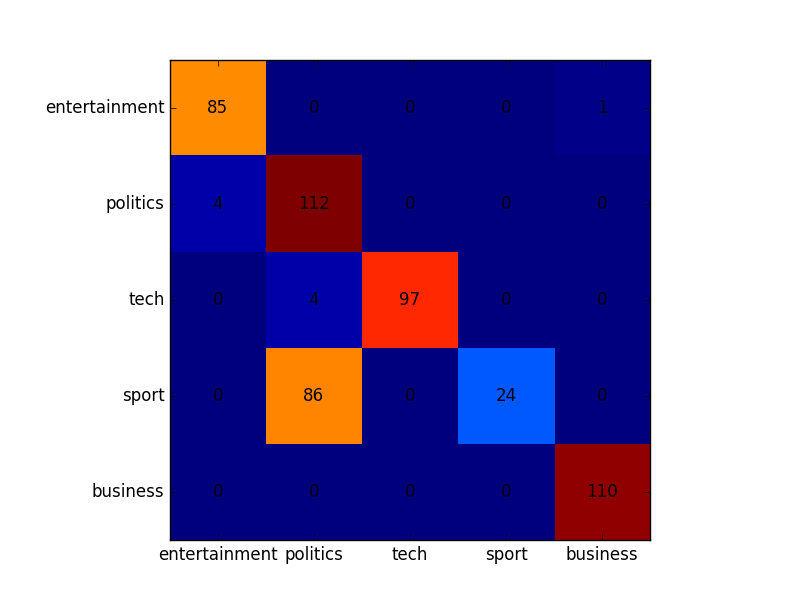
\includegraphics[scale=.4]{conf3.png}
				\caption{Predicted categories v/s Actual categories}
			\end{figure}
			
	\end{frame}
	
	\begin{frame}
			\frametitle{Rules - politics}
			\begin{center}
				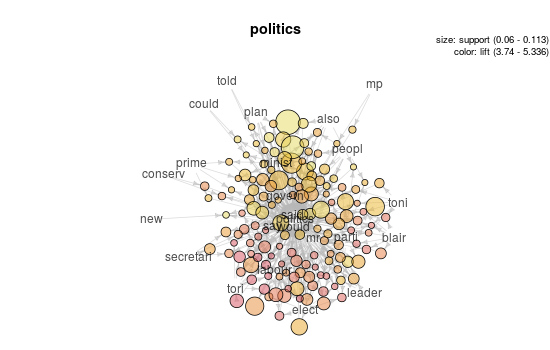
\includegraphics[scale=0.55]{politics.png}
			\end{center}
	\end{frame}
	
	\begin{frame}
			\frametitle{Rules - tech}
			\begin{center}
				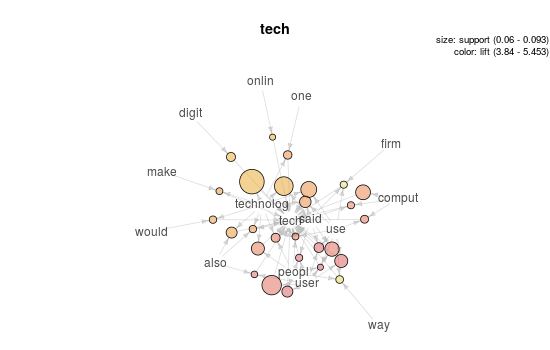
\includegraphics[scale=0.55]{tech.png}
			\end{center}
	\end{frame}
	
	\begin{frame}
			\frametitle{Rules - sport}
			\begin{center}
				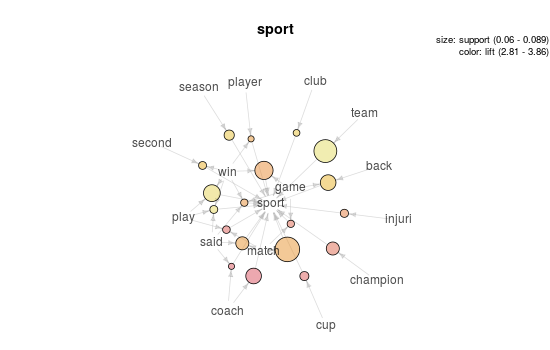
\includegraphics[scale=0.55]{sport.png}
			\end{center}
	\end{frame}
	
	
	\begin{frame}
			\frametitle{Rules - tech}
			\begin{center}
				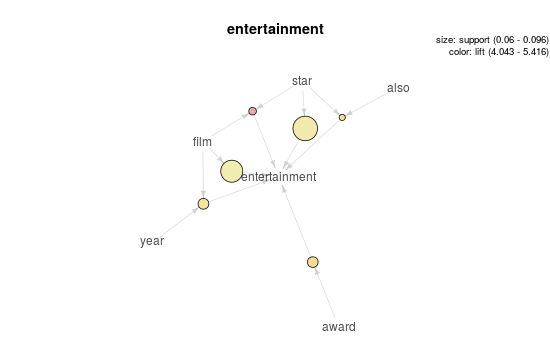
\includegraphics[scale=0.55]{entertainment.png}
			\end{center}
	\end{frame}
	
	\begin{frame}
			\frametitle{Rules - business}
			\begin{center}
				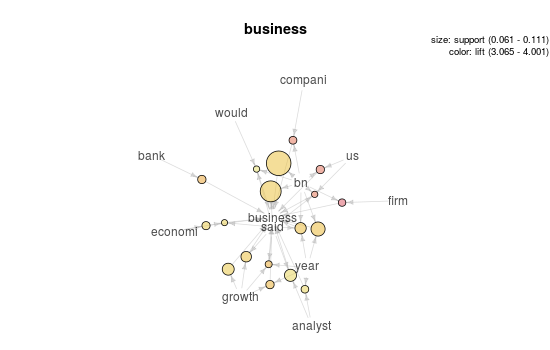
\includegraphics[scale=0.55]{business.png}
			\end{center}
	\end{frame}
	
	\begin{frame}
			\frametitle{Pros}
			\begin {itemize}
			\item Uses existing tools (Apriori Algorithm). 
			\item 50\% to 67\% faster than Apriori.
			\item More transparent than other text classification Algorithms.
			\item Allows domain experts to tune the model.
			\end {itemize}
			
	\end{frame}
	
	\begin {frame}
	\frametitle{Cons}
	\begin {itemize}
			\item Ignores the relative order of terms.
			\item While used for pre-processing, term frequency is not considered for classification.
			\item Parameters (Minimum support, Minimum confidence, Critical Relative support threshold) need to be tuned carefully.
			\end {itemize}
	\end {frame}


	
		\begin{frame}
			\frametitle{References}
			\begin{enumerate}
			\item Rakesh Agrawal and Ramakrishnan Srikant, "Fast algorithms for mining association rules in large databases, Proceedings of the 20th International Conference on Very Large Data Bases, VLDB", pages 487-499, Santiago, Chile, September 1994.
			\item Zailani Abdullah, Tutut Herawan, Noraziah Ahmad and, Mustafa Mat Deris, "Mining significant association rules from educational data using critical relative support approach, Procedia - Social and Behavioral Sciences", 28 (2011) 97 – 101. 
			\item Gayathri, K.; Marimuthu, A., "Text document pre-
processing with the KNN for classification using the
SVM," in Intelligent Systems and Control (ISCO),
2013 7th International Conference on, vol., no.,
pp.453-457, 4-5 Jan. 2013.%
			\seti
			\end{enumerate}
			 
			 
		\end{frame}
		
		\begin{frame}
			\frametitle{References}
			\begin{enumerate}
			\conti
			\item Kadhim, A.I.; Cheah, Yu.-N.; Ahamed, N.H., "Text Document Preprocessing and Dimension Reduction
Techniques for Text Document Clustering," in
Artificial Intelligence with Applications in
Engineering and Technology (ICAIET), 2014 4th
International Conference on , vol., no., pp.69-73, 3-5
Dec. 2014.
			\item D. Greene and P. Cunningham. "Practical Solutions to the Problem of Diagonal Dominance in Kernel Document Clustering", Proc. ICML 2006
			\item Kulkarni, A.R.; Tokekar, V.; Kulkarni, P., "Identifying
context of text documents using Naïve Bayes
classification and Apriori association rule mining," in
Software Engineering (CONSEG), 2012 CSI Sixth International Conference", Sept.2012.
			\seti
			\end{enumerate}
			 
			 
		\end{frame}

\end{document}